\section{Introduction}

Parameterizing a surface amounts to finding a one-to-one mapping from
a suitable domain to the surface. A good mapping is the one which
minimizes either angle distortions (conformal parameterization) or
area distortions (equiareal parameterization) in some sense.  In this
package, we focus on parameterizing triangulated surfaces which are
homeomorphic to a disk, and on piecewise linear mappings onto a planar
domain.

Although the main motivation behind the first parameterization methods
was the application to texture mapping, it is now frequently used for
mapping more sophisticated modulation signals (such as normal,
transparency, reflection or light modulation maps), fitting scattered
data, re-parameterizing spline surfaces, repairing CAD models,
approximating surfaces and remeshing.

This \cgal\ package implements some of the state-of-the-art
surface parameterization methods, such as least squares conformal maps,
discrete conformal map, discrete authalic
parameterization, Floater mean value coordinates or Tutte barycentric
mapping. These methods mainly distinguish by the distortion they
minimize (angles vs. areas), by the constrained border onto the
planar domain (convex polygon vs. free border) and by the guarantees
provided in terms of bijective mapping.

The package proposes currently an interface with \ccc{CGAL::Polyhedron_3<Traits>}
data structure.

Since parameterizing meshes require efficient representation of sparse
matrices and efficient iterative or direct linear solvers, we provide
a unified interface to linear solver libraries (\eigen\ and {\sc Taucs}),
and propose a separate package devoted to OpenNL sparse
linear solver.

Note that linear solvers commonly use double precision floating point
numbers. Therefore, this package is intended to be used with a \cgal\
Cartesian kernel with doubles.

The intended audience of this package is researchers, developers or
students developing algorithms around parameterization of triangle
meshes for geometry processing as well as for signal mapping on
triangulated surfaces.

% Insert image introduction.jpg/eps with title:
% Top: Julius Cesar mask and a checker board texture
% Bottom: Least Squares Conformal Maps parameterization (left: parameter space, right: textured model)
\begin{center}
    \label{Surface_mesh_parameterization-fig-introduction}
    % Image
    \begin{ccTexOnly}
        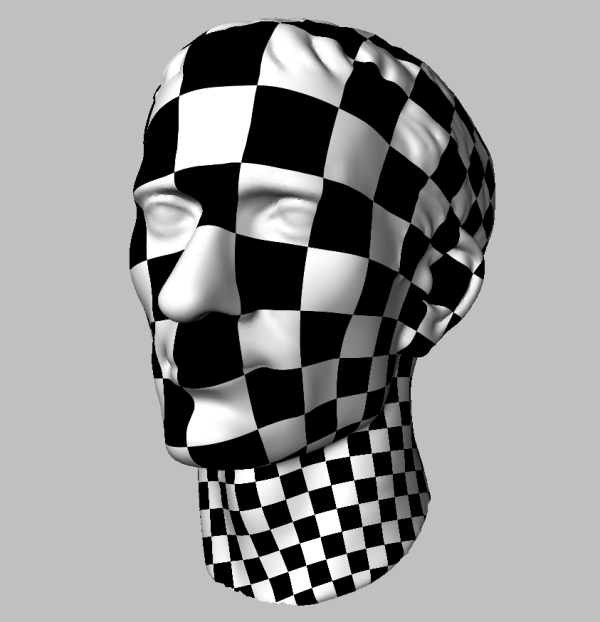
\includegraphics[width=1.0\textwidth]{Surface_mesh_parameterization/introduction} % omit .eps suffix
    \end{ccTexOnly}
    \begin{ccHtmlOnly}
        <img style="max-width: 70%;" border=0 src="./introduction.jpg"><P>
    \end{ccHtmlOnly}
    % Title
    \begin{figure}[h]
        \caption{Texture mapping via Least Squares Conformal Maps parameterization. Top: original mesh and texture. Bottom: parameterized mesh (left: parameter space, right: textured mesh).}
    \end{figure}
\end{center}


